% Kompilieren mit [Strg] + F7
% Ansicht mit F5

\documentclass[12pt]{scrartcl} %Schriftgr��e 12 pt, Art des Dokuments: Kurzartikel

\usepackage{amsmath} %Mathematischer Formelsatz
\usepackage{amssymb} %Einbindung von Sonderzeichen
\usepackage{graphicx} %Erm�glicht das Einbinden von Abbildungen.
\usepackage[latin1]{inputenc} %Kodierung f�r unixoide und Windowssysteme
\usepackage{ngerman} %Bindet die neue deutsche Rechtschreibung ein.
\usepackage{wrapfig} % textumflossene Abbildungen
\usepackage{sidecap} % seitliche Captions
\usepackage{subfigure} % Mehrere Bilder nebeneinander
\usepackage{mathrsfs} % sehr kursive schrift

\begin{document}
	
\begin{titlepage}
\title{\LaTeX-Einf�hrung}
\subtitle{
    Ein Hands-On-Kurs f�r Physik-Studierende an der WWU M�nster
}
\author{
    Pascal Ewen (2011-2012)\\
    Wasilij Barsukow (2011-2013)\\
    Christopher Hodde (2013)
}
\date{14. August 2012}
\end{titlepage}
\maketitle

\newpage
\section{Titelseite}
\label{sec:Titelseite}
Titel, Autor und Datum mit Befehlen \verb+\title{}+, \verb+\author{}+, \verb+\date{}+ innerhalb von \verb+\begin{titlepage}   \end{titlepage}+ setzen, Titelseite mit \verb+\maketitle+ aufrufen.
\\Das heutige Datum erh�lt man mit dem Befehl \verb+\today+.

\newpage
\section{Einfach nur Text}
\label{sec:nurtext}
Man kann in einem \LaTeX-Dokument auch einfach nur Text eingeben. Probiert das einmal! Hier w�re ein kleiner Text zum Ausprobieren:\\\\

{\sl Ob ich mich in diesem Buche zum Helden meiner eignen Leidensgeschichte entwickeln werde, oder ob jemand anders diese Stelle ausf�llen soll, wird sich zeigen. 
\\Um mit dem Beginn meines Lebens anzufangen, bemerke ich, dass ich, wie man mir mitgeteilt hat, und wie ich auch glaube, an einem Freitag um Mitternacht zur Welt kam. Es hei�t, dass die Uhr zu schlagen begann, gerade als ich zu schreien anfing. 
\\Was den Tag und die Stunde meiner Geburt betrifft, so behaupteten die Kindsfrau und einige weise Frauen in der Nachbarschaft, die schon Monate zuvor, ehe wir noch einander pers�nlich vorgestellt werden konnten, eine lebhafte Teilnahme f�r mich gezeigt hatten, erstens: 
\\Dass es mir vorausbestimmt sei, nie im Leben Gl�ck zu haben, und zweitens: 
\\Dass ich die Gabe besitzen w�rde, Geister und Gespenster sehen zu k�nnen. Wie sie glaubten, hingen diese beiden Eigenschaften unvermeidlich all den ungl�cklichen Kindern beiderlei Geschlechts an, die in der Mitternachtsstunde eines Freitags geboren sind. 
\\�ber den ersten Punkt brauche ich nichts weiter zu sagen, weil ja meine Geschichte am besten zeigen wird, ob er eingetroffen ist oder nicht. Was den zweiten anbelangt, will ich nur feststellen, dass ich bisher noch nichts bemerkt habe.
\\\phantom{a}\hfill Charles Dickens, David Copperfield}
\\\\
Ein Zeilenumbruch entsteht erst durch Einf�gen von \verb+\\+ oder \verb+\newline+ (gleichwertig). Ein Seitenumbruch funktioniert mit \verb+\newpage+.

Die Befehle \verb+\LaTeX+ und \verb+\TeX+ sind selbsterkl�rend. Bitte achtet auf Gro�- und Kleinschreibung! Kommentare (Text, der, sollte er sogar Befehle enthalten, trotzdem nicht von \LaTeX~interpretiert wird) beginnen mit \verb+%+. Sie erstrecken sich stets bis zum Ende der Zeile.

Es ist l�stig, riesige Dokumente zu verwalten. Dazu gibt es den \verb+\input+-Befehl.
\begin{itemize}
	\item Legt daf�r eine leere Datei an, gebt ihr einen vern�nftigen Namen und die Endung \verb+.tex+.
	\item Schneidet euren getippten Text aus der Hauptdatei aus und legt ihn in der neu erstellten Datei ohne irgendwelche weiteren Befehle ab.
	\item Schreibt in euer Hauptdokument an die Stelle des Textes \verb+\input{hier pfad}+. Der Pfad kann relativ sein, d. h. es gen�gt schon allein der Dateiname (mit oder ohne Endung), wenn die Dateien im gleichen Ordner liegen. In der Ordnerstruktur hinauf bewegt man sich mit \verb+../+
\end{itemize}
Bitte verwendet solche Auslagerungen!

\newpage
\section{Befehle in \TeX}
\label{sec:befehle}
Jeder Befehl in \LaTeX~beginnt mit einem backslash $\backslash$. Man kann/muss manchen Befehlen etwas mitteilen: z. B. bei \verb+\title+, man spricht dann von �bergabeparametern. Wenn der Befehl einen Parameter erwartet, sucht er ihn direkt hinter dem Befehlsbezeichner. 

Um zu verstehen, wozu Klammerung mit \{ \} gut ist, probiert doch einmal die beiden Befehle: \verb+\title Buchtitel+ und \verb+\title{Buchtitel}+. \LaTeX~nimmt sich immer die erste Gruppe als Parameter. Eine Gruppe w�re entweder etwas, was zwischen \verb+{+ und \verb+}+ steht, oder ein Befehl oder ein Buchstabe. Im ersteren Fall w�rde also als Titel nur das \verb+B+ genommen und \verb+uchtitel+ als darauf folgender Text interpretiert. \verb+\titleBuchtitel+ (ohne Leerzeichen) wird nicht funktionieren, da \TeX~nicht erkennt, wo der Befehl enden und der Parameter anfangen soll.
\\\scriptsize Man spricht hier vom {\sl befehlstrennenden Leerzeichen}. Dieses ist wichtiger als man zun�chst glaubt. Dazu vergleiche man die Ausgaben der vier S�tze: \\\verb+Ich mag \LaTeXsehr.+, \newline\verb+Ich mag \LaTeX sehr.+, \newline\verb+Ich mag \LaTeX    sehr.+ und \newline\verb+Ich mag \LaTeX~sehr.+. Die Tilde \verb+~+ ist ein Leerzeichen, an dem die Zeile nicht umgebrochen werden darf. Man setzt es eigentlich z. B. bei Namen und Titeln: \verb+Dr.~M�ller+. \normalsize

\newpage
\section{Mathematische Formelumgebung}
\label{sec:MathematischeFormelumgebung}

\LaTeX~erlaubt keine mathematischen Zeichen im gew�hnlichen Text, man muss daf�r in eine \textbf{mathematische Umgebung} wechseln. Ihrer gibt es  etwa ein halbes Dutzend, je nach Zweck verwendet man die eine oder andere. Aktiv nutzt man gew�hnlich jedoch nur zweieinhalb. Wir behandeln hier:
\begin{itemize}
	\item \verb+\begin{equation} ... \end{equation}+
	\item \verb+\begin{align} ... \end{align}+ --  nummerierte und ausgerichtete Gleichungsfolge
	\item \verb+$ ... $+ -- eingebettete Formel
\end{itemize}

\newpage 
\subsection{Nummerierte Gleichung}
\label{sec:NummerierteGleichung}
% equation
{\sl Nur} im Mathematik-Modus, d. h. innerhalb der drei Umgebungen funktionieren die zahlreichen Mathematik-Befehle. F�r
\begin{equation}
	E = mc^2
\end{equation}
gibt man ein:\\
\verb+\begin{equation} E = mc^2 \end{equation}+\\
Leerzeichen und Zeilenumbr�che sind egal! N�tzliche Allerwelts-Befehle: 
	\begin{itemize}
		\item \verb+a^n+ ergibt $a^n$
		\item \verb+\frac{a}{b}+ ergibt $\frac{a}{b}$
		\item \verb+n_i+ ergibt $n_i$
		\item \verb+\cdot+ ergibt den Malpunkt $\cdot$ (\emph{bitte nie * benutzen!}) 
		\item \verb+\sqrt{abc}+ ergibt Wurzel: $\sqrt{abc}$.
		\item (Fast) alle griechischen Buchstaben erreicht man mit $\backslash $ Plus ausgeschriebenen Namen, z. B. \verb+\pi+, \verb+\alpha+, \verb+\theta+. Gro�buchstaben werden gro� geschrieben: \verb+\Pi+, \verb+\Theta+. Warum gibt es kein \verb+\Alpha+?
	\end{itemize}
	{\scriptsize Das \verb+c+ steht f�r {\sl center}. Man darf gerne schon jetzt \verb+ldots+ und \verb+ddots+ ausprobieren, sie kommen aber zusammen mit \verb+\dot+ etwas sp�ter.}

Mit \verb+\frac{a}{b}+ lernen wir einen Befehl kennen, der zwei Argumente erwartet. Vergleicht die Ausgabe von \verb+\frac{a}{b}+ mit der von \verb+\frac a b+ und \verb+\frac ab+! Was passiert, wenn man \verb+\frac pV T = const+ eingibt?

Wichtig: Keinerlei Leer\emph{zeilen} in den mathematischen Umgebungen!\\
Zur �bung: 
\begin{equation} F = -G \cdot \frac{mM}{r^2} \end{equation}
\begin{equation} C = \frac{Q}{U}\end{equation}
\begin{equation} U = U_0 \cdot e^{-\frac{t}{RC}}\end{equation}
\begin{equation} U = 2 \pi r\end{equation}
\begin{equation} A = \pi r^2 = \pi \frac{d^2}{4}\end{equation}
\begin{equation} r = \sqrt{\frac{(s-a)(s-b)(s-c)}{s}}\end{equation}

Gleichungen erhalten hier automatisch Nummern. Um auf diese Nummer zu verweisen verwende man sie auf keinen Fall explizit! Ver�ndert sich n�mlich weiter oben etwas, muss man alle Nummern per Hand �ndern. Das ist nicht n�tig, da \LaTeX~schon selbst darauf achtet. Wie �berall sonst auch (Bilder, Tabellen, Kapitel, ...: dieses System bezieht sich nicht nur auf Gleichungen!) heftet man einem Objekt ein \verb+\label{hier name des labels}+ an und kann dann �ber diesen (frei w�hlbaren) Namen mithilfe von \verb+\ref{hier name des labels}+ stets die aktuelle Nummer abrufen. F�r die �bliche Klammerung dieser muss man selbst sorgen\footnote{Nat�rlich nicht! Zum einen gibt es verbesserte Varianten der Referenzierung, wo die Klammerung schon enthalten ist, und des Weiteren kann man sich nat�rlich selbst einen Befehl definieren, der nichts anderes macht, als die Klammern zu setzen und dazwischen den urspr�nglichen aufzurufen.}.

\begin{equation}
	E = mc^2
	\label{eq:energie}
\end{equation}
Sp�ter im Text verweist man dann auf Gleichung (\ref{eq:energie}).

Daf�r einzugeben:\\
\verb+\begin{equation}+\\
\verb+    E = mc^2+\\
\verb+    \label{eq:energie}+\\
\verb+\end{equation}+\\
\verb+Sp�ter im Text verweist man dann auf Gleichung (\ref{eq:energie}).+\\

Man beachte, dass \LaTeX~beim ersten Kompilieren zun�chst die ganzen \verb+\label+s liest, und beim zweiten Kompilieren erst die \verb+\ref+-Referenzen interpretieren kann. Bis dahin werden sie als (??) ausgef�llt -- nicht erschrecken, sondern noch einmal laufen lassen! �brigens gibt es dazu jedes Mal eine amtliche Warnung: \emph{LaTeX Warning: Label(s) may have changed. Rerun to get cross-references right.}

Meist will man aber nicht nur eine Gleichung haben, sondern mehrere untereinander, z. B. als Zwischenschritte einer Herleitung. Die Gleichungen sollen vern�nftig ausgerichtet werden.

\newpage
\subsection{Gleichungsfolge}
\label{sec:Gleichungsfolge}
% align

Am h�ufigsten verwendet man wohl beim Schreiben die Umgebung \newline \verb+\begin{align} hier viele Formeln \end{align}+.
\begin{itemize}
	\item Sie nummeriert ihre Gleichungen automatisch (Wenn man allerdings auf Gleichungen verweisen will, muss man trotzdem per Hand jede davon mit einem \verb+\label+ versehen.)
	\item Nummerierungen schaltet man grunds�tzlich in allen solchen Umgebungen ab, indem man hinter den Namen der Umgebung ein * schreibt: \verb+align+ $\rightarrow$ \verb+align*+, \verb+equation+ $\rightarrow$ \verb+equation*+.
	\item Es d�rfen (und sollen) Zeilenumbr�che \verb+\\+ verwendet werden.
	\item Wenn man vor einem Symbol ein \verb+&+ verwendet, wird an diesem Symbol ausgerichtet.
\end{itemize}
Beispiel:
\begin{align*}
	(a + b)^2 &= (1 + (a-1) + b)^2\\
						&= (1 + 1 + (a-2) + b)^2\\
						&= (1 + 1 + 1 + (a-3) + b)^2
\end{align*}
Weiterhin werden jegliche Leerzeichen und Tabulatoren ignoriert. Die Tabulatoren im Code dienen nur der Leserlichkeit desselben!\\
\verb+\begin{align*}+\\
\verb!   (a + b)^2 &= (1 + (a-1) + b)^2\\!\\
\verb!             &= (1 + 1 + (a-2) + b)^2\\!\\
\verb!             &= (1 + 1 + 1 + (a-3) + b)^2!\\
\verb!\end{align*}!

Probieren wir wieder ein paar neue Befehle (Hier wurden insgeheim \verb+\limits+ und \verb+\displaystyle+ verwendet):
\begin{itemize}
	\item \verb+\sum_{i=0}^{\infty}+ ergibt $\displaystyle \sum_{i = 0}^{\infty}$
	\item \verb!\int_{-\infty}^{+\infty}! ergibt $\displaystyle \int\limits_{-\infty}^{+\infty}$
	\item \verb+\vec a+ ergibt $\vec a$
	\item \verb+\dot a+ ergibt $\dot a$, \verb+ddot a+ -- $\ddot a$.
\end{itemize}

\newpage
\subsection{�bung dazu}
\label{sec:uebung1}
Schreibt diese Formeln: 
\begin{align*}
	0 &= \frac{1}{\pi} \int_0^{2 \pi} \cos (nx) \sin (mx) \: dx\\
	\dot Q &= - \lambda A \frac{\Delta T}{L}\\
	\vec I &= \int_V \vec j \: d V\\
	\vec F &= - \frac{1}{4 \pi \varepsilon_0} \frac{q_1q_2}{|\vec r_1 - \vec r_2|^3} (\vec r_1 - \vec r_2)
\end{align*}
Wichtig: Keinerlei Leer\emph{zeilen} in den mathematischen Umgebungen!\\
Verwende nun \verb+\label+-\verb+\ref+.
\begin{align}
	\vec \nabla \cdot \vec \jmath + \frac{\partial}{\partial t} \rho &= 0\\
	\vec \nabla \cdot \vec B &= 0 \label{eq:divB}\\
	\vec \nabla \cdot \vec E &= \frac{\rho}{\epsilon_0} \label{eq:divE}
\end{align}
Der Befehl \verb+\int+ erwartet als (optionale!) Parameter die Grenzen, nicht den Integranden! Hinweis: Verwende \verb+\partial+ f�r $\partial$ und \verb+\nabla+ f�r $\nabla$.\\
So verwendet man dann die Referenzen:\\
{\sl Der Unterschied zwischen den Gleichungen (\ref{eq:divB}) und (\ref{eq:divE}) liegt in der experimentell festgestellten Nicht-Existenz magnetischer Monopole. Aus Gleichung (\ref{eq:divE}) l�sst sich das Coulomb-Gesetz herleiten.}

\subsection{Eingebettete Formel}
\label{sec:EingebetteteFormel}

Hier ist ganz viel Text und noch mehr Text und noch viel mehr Text und mitten im Text, zum Beispiel hier: $a^2 + b^2 = c^2$ steht eine Formel! Ist sie nicht wundersch�n? Dazu muss einfach \verb-$a^2 + b^2 = c^2$- eingegeben werden!

Innerhalb der Dollarzeichen \verb+$ $+ befindet man sich in der gleichen mathematischen Umgebung wie sonst auch. Die Formel wird aber im Text belassen.
\begin{itemize}
	\item Alle mathematischen Befehle sind \emph{ausschlie�lich} im Mathematik-Modus erreichbar. Manchmal braucht man einen griechischen Buchstaben auch im Text, trotzdem muss man in den mathematischen Modus wechseln: den Text 
	
	"`das griechische Alphabet ist mehrere Tausend Jahre alt, es besteht aus den Kleinbuchstaben $\alpha, \beta, \gamma, \delta, \epsilon, ...$ und den Gro�buchstaben A, B, $\Gamma$, $\Delta$, E, ..."' 
	
	erh�lt man durch Eingabe von 
	
	\verb+"`das griechische Alphabet ist mehrere Tausend Jahre alt, es+ \\\verb+besteht aus den Kleinbuchstaben $\alpha$, $\beta$, $\gamma$, $\delta$,+ \\\verb+$\epsilon$, ... und den Gro�buchstaben A, B, $\Gamma$, $\Delta$, E, ..."'+
	\item Im Mathematik-Modus werden Leerzeichen generell missachtet: \verb+$a     b$+ ergibt als Ausgabe $a     b$.
	\item Das \verb+\label{}+ kann man einer \verb+$+-Umgebung nicht anheften.
	\item Bitte schreibt im Text \textbf{nie} etwas von einer x-Achse, sondern stets nur von der $x$-Achse. (\verb+x-Achse+ $\leftrightarrow$ \verb+$x$-Achse+)
	\item Da \emph{in} der Zeile wenig Platz ist, eignet sich die \verb+$ ... $+-Umgebung mit steigender vertikalen Ausdehnung der Br�che immer weniger.
\end{itemize}

\newpage
\subsection{Zwischenstand}
\label{sec:zwstand2}

�bersicht:
\begin{itemize}
	\item symbolhaft:
		\begin{itemize}
			\item \verb+$ ... $+
		\end{itemize}
		gut f�r unwichtige Formeln bzw Variablen und kleine Terme im Text
	\item echte Umgebungen (\verb+\begin+, \verb+\end+)
		\begin{itemize}
			\item \verb+equation+
			\item \verb+align+
		\end{itemize}
		gut f�r gro�e Rechnungen, nummerierbar. Nat�rlich kann man auch in \verb+align+ eine einzige Gleichung schreiben!
	\item Kleine Tricks: 
		\begin{itemize} 
			\item Es gibt eine M�glichkeit, in einer \verb+align+-Umgebung nicht alle Gleichungen mit einer Nummer zu versehen, sondern nur diejenigen, die tats�chlich ein \verb+\label+ tragen. Dazu ist folgendes bei den \verb+package+-Einbindungen hinzuzuf�gen:
				\\\verb+\usepackage{mathtools}+
				\\\verb+\mathtoolsset{showonlyrefs}+
			\\Der gebrauchten Gleichung heftet man wie gewohnt ein \verb+\label{}+ an, der Verweis erfolgt aber mit \verb+\eqref{...}+ ohne runde Klammern, denn diese sind jetzt schon automatisch dabei.
			\item In der \verb+align+-Umgebung f�gt \LaTeX~keinen Seitenumbruch ein (eines der Probleme damit...)
		\end{itemize}
\end{itemize}

\newpage
\subsection{H�ufige mathematische Symbole}
\label{sec:GrundlegendeMathematischeBegriffe}

Grunds�tzlich gilt: Alles was man nicht beh�lt, kann man stets nachgucken. Alle Befehle zu kennen ist unm�glich (eine fast allumfassend scheinende, aber sicher immer noch nicht vollst�ndige Auswahl wird regelm��ig von "`amtlichen"' Stellen publiziert und umfasst im Moment 164 Seiten\footnote{http://www.tex.ac.uk/tex-archive/info/symbols/comprehensive/symbols-a4.pdf}). Eine erste Anlaufstelle ist \verb+Hilfe:TeX+ bei wikipedia (genau so in die Suche eingeben). Auf vielen Foren wurden auch schon zahlreiche Probleme diskutiert.

Eine kleine �bersicht, was alles geht:
\subsubsection{gro�e Symbole}
	\begin{itemize}
		\item $\displaystyle\sum_{i=0}^n$ mit \verb+\sum_{i=0}^n+\\
		\item $\displaystyle\int_a^b$ mit \verb+\int_a^b+\\
		\item $\displaystyle\frac{a + b}{b}$ mit \verb-\frac{a + b}{b}-
		\item $\displaystyle\sqrt[3]{8} \sqrt{5}$ mit \verb+\sqrt[3]{8} \sqrt{5}+\\
	\end{itemize}
\subsubsection{buchstabengro�e Symbole}
	\begin{itemize}
		\item $abcdefghijklmnopqrstuvwxyz$
		\item F�r $\jmath$ statt $j$ und $\imath$ statt $i$ verwende man \verb+\jmath+ und \verb+\imath+. Mit Vektorpfeil sieht $\vec \jmath$ einfach besser aus!
		\item $ABCDEFGHIJKLMNOPQRSTUVWXYZ$
		\item $\alpha \beta \gamma \delta \epsilon \zeta \eta \theta \iota \kappa \lambda \mu \nu \xi o \pi \rho \sigma \tau y \phi \chi \psi \omega$
		\item Vergleiche: $\epsilon\leftrightarrow\varepsilon$, $\theta\leftrightarrow\vartheta$, $\rho\leftrightarrow\varrho$ , $\phi\leftrightarrow\varphi$. Die Abwandlungen entstehen durch Voranstellen von \verb+var+: \verb+\varepsilon, \vartheta, \varrho, \varphi+.
		\item $\infty$, $\nabla$, $\partial$, $\hbar$ mit \verb+$\infty$, $\nabla$, $\partial$, $\hbar$+.
\end{itemize}

	\subsubsection{Schrift}
	Formeln werden stets kursiv angezeigt. Will man ein St�ck Text darin haben, verwende man \verb+\text{hier der text}+: $\displaystyle \frac{\text{Zaehler}}{\text{Nenner}} \neq  \frac{Zaehler}{Nenner}$ (\verb+\frac{\text{Zaehler}}{\text{Nenner}}+).
	
	Zudem gibt es verschiedene, speziell f�r die Mathematik erfundene Schriftarten:
	\begin{itemize}
		\item \verb+\mathcal{HIER SYMBOL}+: $\mathcal{ABCDEFGHIJKLMNOPQRSTUVWXYZ}$ (nur Gro�buchstaben!)
		\item \verb+\mathbb{HIER SYMBOL}+: $\mathbb{ABCDEFGHIJKLMNOPQRSTUVWXYZ}$ (nur Gro�buchstaben!)
		\item \verb+\mathscr{HIER SYMBOL}+: $\mathscr{ABCDEFGHIJKLMNOPQRSTUVWXYZ}$ (nur Gro�buchstaben!, mit dem \verb+mathrsfs+-package)
	\end{itemize}
	
	\subsubsection{Konjunktionen, Erweiterungen}
		\begin{itemize}
			\item $a^b$, $a_b$ mit \verb+$a^b$, $a_b$+
			\item $\cdot$, $\cdots$, $\vdots$, $\ddots$, $\ldots$ mit \newline \verb+$\cdot$, $\cdots$, $\vdots$, $\ddots$, $\ldots$+
			\item $>$, $<$, $\leq$, $\geq$, $\neq$, $\ll$, $\gg$, $\propto$, $\approx$, $\equiv$ mit \newline \verb+$>$, $< $, $\leq$, $\geq$, $\neq$, $\ll$, $\gg$, $\propto$, $\approx$, $\equiv$+
			\item $\rightarrow$, $\Rightarrow$, $\leftrightarrow$, $\Leftrightarrow$, $\to$, $\mapsto$ mit \newline \verb+$\rightarrow$, $\Rightarrow$, $\leftrightarrow$, $\Leftrightarrow$, $\to$,+ \\ \verb+$\mapsto$+
			\item $\vec a$, $\dot a$, $\bar a$, $\hat a$, auch kombiniert: $\dot{\vec v}$ mit \newline \verb+$\vec a$, $\dot a$, $\bar a$, $\hat a$, $\dot{\vec v}$+
		\end{itemize}

\newpage
\subsection{Mathematische Formatierungsregeln}
\label{sec:MathematischeFormatierungsregeln}

	\subsubsection{Gruppierung}
	Frage: Was passiert, wenn man \verb+10^-10+ eingibt? \verb+U_ind+?
	
	\subsubsection{Funktionennamen u�}
	Variablen werden grunds�tzlich kursiv gesetzt. Dies ist auch gebr�uchlich. Bitte schreibt im Text \textbf{nie} etwas von einer x-Achse, sondern stets nur von der $x$-Achse. Und so weiter.
	
	Doch gibt es F�lle, wo dies nicht erw�nscht ist: $sin x$ sieht entsetzlich aus! Deswegen:
		\\F�r die meisten Funktionen schreibe man vor den Funktionsnamen ein $\backslash$: \verb+sin x+ $\to$ \verb+\sin x+, \verb+log x+ $\to$ \verb+\log x+, usw.
		
		Es ist auch un�blich, bestimmte Indizes kursiv zu setzen: Vergleiche $U_{ind}$ mit $U_{\text{ind}}$, $R_{eff}$ mit $R_{\text{eff}}$ (Ligatur\footnote{Vergleiche $fi$ mit fi.}!) usw. Generell gilt: Bezieht sich der Index auf eine Variable, wie etwa in $n_k \quad k \in \{1, 2, \ldots, N \}$, so ist der Index als Variable, also kursiv zu setzen. Bezieht sich der Index auf ein Wort oder einen Namen, wie in der Fermi-Energie, so ist $E_\text{F}$ anstatt von $E_F$ zu setzen.
		
		Schreibe: $$ A = \frac{\tan x \sin x}{\pi^2 \varrho_{\text{neu}}} \cdot \varrho_{\text{alt}} \cdot \int_1^X \exp \left (  \frac{m v^2}{2\ln x} \right) \: dx$$
		
		Falls einmal ein Name nicht enthalten ist (z. B. \verb+\span+), so schreibe man doch statt \verb+$span$+ wenigstens \verb+\text{span}+: $span_{\mathbb{K}} \to \text{span}_{\mathbb{K}}$.
		
		Schreibe das als �bung! (Puristen\footnote{Die zugeh�rigen DIN Normen tragen Nummern ab 1300.} bestehen auch auf $\text{d}x$ statt $dx$)
	
	\subsubsection{Klammern}
		\LaTeX~setzt auch selbst die Gr��e der Klammern, nur nicht automatisch. Dazu muss man ihn darauf hinweisen, dass er bitte selbst alles erledigen soll. Beispiel: $$(\frac{1}{R_0} - \frac{1}{r})$$ oder $$|\frac{a}{b}|$$ Sollen zwei Begrenzer so in ihrer Gr��e angepasst werden, dass alles genau passt, so schreibe man \emph{vor} den linken \verb+\left+ und \emph{vor} den rechten \verb+\right+.
		
		Schreibe das als �bung: $$\left (\frac{1}{R_0} - \frac{1}{r} \right)$$ $$\left |\frac{a}{b} \right|$$

	\subsubsection{Abst�nde}
		Manchmal ist es n�tig, die automatische Abstandssetzung von \LaTeX~zu korrigieren, etwa hier: $\int xdx \to \int x \: dx$. Dazu gibt es diese Befehle (die man nicht allzu h�ufig benutzen sollte):
		\begin{itemize}
			\item \verb+\,+, \verb+\:+ -- ein (sehr) kleiner Abstand (schmales Leerzeichen)
			\begin{itemize}
				\item Es ist guter Stil, zwischen Zahl und Einheit ein schmales Leerzeichen zu setzen. Vergleiche: $230 V$, $230\text{ V}$, $230\,\text{V}$
			\end{itemize}
			\item \verb+\enspace+ -- so breit wie eine Ziffer
			\item \verb+\quad+ -- so breit, wie ein Buchstabe hoch ist
			\item \verb+\qquad+ -- doppelt so breit wie ein \verb+\quad+
			\item \verb+\!+ -- Ein negativer Abstand, um Zeichen nach links zu r�cken
		\end{itemize}
		
	\newpage
\section{Textformatierung}
\label{sec:Textformatierung}
  Zur Textformatierung gibt es nur wenige, daf�r aber sehr effiziente Befehle:\\
  Schriftgr��e:
  \begin{itemize}
  	\item \verb+\tiny+
  	\item \verb+\small+
  	\item \verb+\large+
  	\item \verb+\Large+
  	\item \verb+\huge+
  	\item \verb+\Huge+
  	\item Ganz wichtig: \verb+\normalsize+
  \end{itemize}
  {\tiny Das ist }{\small ein Satz, }{\large der }{\Large diese } {\huge Schriftgr��en demonstriert.}

	Beachte, dass diese Befehle solange gelten, bis eine neue Schriftgr��e angegeben wird\footnote{Das stimmt nicht ganz: Sie gelten nur bis zum Ende des Gruppierungsblocks.}. Im Allgemeinen braucht man diese Befehle nur, wenn man nicht die \LaTeX-eigene Gliederungsstruktur verwendet.

	Schiftarten:
	\begin{itemize}
		\item \verb+\textbf{}+ -- \textbf{fett}
		\item \verb+\textit{}+, \verb+\emph{}+ -- \textit{kursiv}
		\item \verb+\textsl{}+ -- \textsl{schief}
		\item \verb+\textsc{}+ -- \textsc{Kapit�lchen}
		\item \verb+\texttt{}+ -- \texttt{Schreibmaschine}
		\item \verb+\underline{}+ -- \underline{unterstrichen}
	\end{itemize}
	 %Wasilij Barsukow und Pascal Ewen
	\newpage	
 	\section{Gliederung}
\label{sec:Gliederung}

	Einen neuen Abschnitt erzeugt man mit dem Befehl \verb+\section{}+.
	Um Schriftgr��en, Zeilenabst�nde und Fettsatz brauch man sich dabei nicht zu k�mmern; die findet \LaTeX von selbst.
	Nat�rlich sind auch tiefere Gliederungen m�glich.
	F�r einen ...

\subsection{Unterabschnitt}
\label{sec:Unterabschnitt}

	gibt es den Befehl \verb+\subsection{}+. F�r einen ...

\subsubsection{Unter-Unterabschnitt}
\label{sec:UnterUnterabschnitt}

	ist \verb+\subsubsection{}+ vorgesehen.


\paragraph{Paragraphen}
\label{sec:Paragraphen}
	lassen sich mit \verb+\paragraph{}+ erzeugen.
\subparagraph{Unter-Paragraphen}
\label{sec:Unter-Paragraphen}
	gibt es auch. Der Befehl lautet \verb+\subparagraph{}+
	Wie man sieht, werden diese standardm��ig nicht nummeriert und nach ihnen wird nicht umgebrochen.
	Auch Gliederungsebenen k�nnen ein \verb+\label{}+ erhalten, sodass man sp�ter zum Beispiel mit \verb+\ref{sec:Unterabschnitt}+ auf Abschn. \ref{sec:Unterabschnitt} verweisen kann.
	
	Schlie�lich sollten lange Flie�texte mittels Abs�tzen etwas aufgelockert werden, um nicht vor dem Auge zu verschwimmen.
	Dazu verwendet man eine \textit{Leerzeile} im Quelltext.
	
\subsection{Liste der Gliederungsebenen}
 \label{sec:Liste der Gliederungsebenen}
	
	Der Vollst�ndigkeit halber noch einmal alle Gliederungsebenen, die zur Verf�gung stehen:
	\begin{itemize}
	
		\item	\verb+\part{}+
		\item	\verb+\chapter{}+ (Funktioniert in einem \verb+scartcl+-Dokument nicht)
		\item	\verb+\section{}+
		\item	\verb+\subsection{}+
		\item	\verb+\subsubsection{}+
		\item	\verb+\paragraph{}+
		\item	\verb+\subparagraph{}+		
	
	\end{itemize}
	
\subsection{�ber Gliederungen}
 \label{sec:Ueber Gliederungen}
	
	Gliederungen und Inhaltsverzeichnisse sind kein Selbstzweck!
	Sie sollen dem Leser �berblick und Orientierung bieten.
	Darum gilt: Ausreichend, aber nicht unn�tig tief und vor allem einheitlich Gliedern.
	
	Sollte man tats�chlich einmal bis zur vierten oder f�nften Ebene nummeriert gliedern wollen, kann man mit dem Schalter
	\verb+\setcounter{secnumdepth}{4}+ die Nummerierungstiefe anpassen und mit \verb+\setcounter{tocdepth}{4}+ die tieferen Ebenen ins Inhaltsverzeichnis aufnehmen:
	\setcounter{secnumdepth}{4}
	\setcounter{tocdepth}{4}
	\paragraph{Nummerierter Paragraph} ~\\
	Dann trickst man \LaTeX noch mit einem gesch�tzten leerzeichen vor dem manuellen Zeilenumbruch: \verb+~\\+ aus und alles sieht so aus, wie es sein soll.

	

	

\newpage
\section{Aufz�hlungen}
\label{sec:Aufzaehlungen}

\subsection{Einfache Aufz�hlung}
\label{sec:EinfacheAufzaehlung}

	Eine einfache Aufz�hlung von Stichpunkten ist im Quelltext in den Block\\
	\begin{verbatim}
		\begin{itemize}
			
			\item
			Erster Aufz�hlungspunkt
			
			\item
			N�chster Aufz�hlungspunkt
			
		\end{itemize}
	\end{verbatim}
	eingeschlossen. Beliebig viele \verb+\item+-s lassen sich zu einer Aufz�hlung zusammenfassen. 
	\begin{itemize}
			
			\item
			Erster Aufz�hlungspunkt
			
			\item
			N�chster Aufz�hlungspunkt
			
		\end{itemize}

\subsection{Nummerierte Aufz�hlung}
\label{sec:nummmerierteAufzaehlung}

	Um die Aufz�hlung durchzunummerieren, verwendet man die Umgebung \\ \verb+\begin{enumerate} ... \end{enumerate}+.
	Jedes Item kann wieder eine \verb+enumerate+-Umgebung enthalten.

\begin{enumerate}
			
			\item
			Erster Aufz�hlungspunkt
			
			\item
			Zweiter Aufz�hlungspunkt
				
			\begin{enumerate}
				\item Unterpunkt Zwo Anton
				\begin{enumerate}
					\item Kleine r�mische Ziffern! 
					\begin{enumerate}
						\item Dies ist leider die tiefstm�gliche Aufz�hlungsebene
					\end{enumerate}				
				\end{enumerate}
			\end{enumerate}
			
			
\end{enumerate}

	Die M�glichkeit, die Art der Nummerierungen jeder Ebene individuell festzulegen, bietet \verb+\usepackage{enumerate}+.
	Dann wird die Art der Nummerierung in eckigen Klammern angegeben, z.B.:\verb+\begin{enumerate}[a)]+ angegeben.
	Verf�gbar sind:
\begin{description}
	\item[1] arabische Nummern
	\item[a] kleine lateinische Buchstaben
	\item[A] gro�e lateinische Buchstaben
	\item[i] kleine r�mische Nummern
	\item[I] gro�e r�mische Nummern
\end{description}
	Jedes Element der obigen Liste kann mit beliebigen Sonderzeichen umgeben werden.


\subsection{Beschreibung}
\label{sec:Beschreibung}

	Die Umgebung \verb+\begin{description}...\end{description}+ erlaubt die Beschreibung von Stichw�rtern, die als \verb+\item[Stichwort]+ gegeben werden.

\begin{description}
	\item[Rekursion] Einer von vielen rekursiven Aufrufen
	\item[rekursiv] Eigenschaft einer auf Rekursionen basierenden Rechung oder Definition
	\item[Endlosschleife] Kann mir nicht passieren
\end{description}



\newpage
\section{Gleitobjekte}
\label{sec:Gleitobjekte}
	
\subsection{Abbildungen}
\label{sec:Abbildungen}

\subsubsection{Einfache Abbildung}
\label{sec:EinfacheAbbildung}

	Nat�rlich m�chten wir auch Abbildungen in unsere Texte einf�gen k�nnen.
	%Daf�r eignet sich das Package \verb+graphicx+, dass wir oben eingebunden haben.
	Meistens m�chten wir sie nicht mitten im Text
	
\includegraphics[height=1em]{Fig1.pdf}
	stehen haben, sondern als einzelne Objekte frei auf dem Blatt verschieben k�nnen.
	M�glich macht es die \verb+figure+-Umgebung:	
\begin{verbatim}
\begin{figure}[h!]
    \centering
        
\includegraphics[width=0.2\textwidth]{Fig1.pdf}
    \caption{Dies ist eine Sonne}
    \label{fig:Fig1}
\end{figure}
\end{verbatim}
%
\begin{figure}[h!]
	\centering
		
\includegraphics[width=0.3\textwidth]{Fig1.pdf}
	\caption{Dies ist eine Sonne}
	\label{fig:Fig1}
\end{figure}
%
	Die wichtige Zeile ist \verb+\includegraphics[Optionen]{Pfad}+.
	Mit den Optionen wird die Gr��e bestimmt. Es geht nat�rlich auch eine Bestimmung \`a la \verb+[height=0.5\textheight]+.
	Wenn die Seitenverh�ltnisse egal sind, kann man auch Breite \textbf{und} H�he festlegen. Der Pfad kann absolut oder relativ angegeben werden.
	
	Der Schalter \verb+\centering+ ist Optional, aber �blich; die Figure-Umgebung belegt sowieso die ganze Breite des Blattes.
	Die Nummerierung der \verb+\caption{}+ erfolgt automatisch. Dank des \verb+labels+ k�nnen wir wie auf Formeln und alle anderen Objekte nun auf Abb.~\ref{fig:Fig1} verweisen.

	Die Platzierung auf der Seite erledigt \LaTeX so, dass die Seiten m�glichst gleichm��ig mit Text gef�llt werden.
	Es richtet sich aber nach den Platzierungsvorgaben:
\begin{description}
\item[h] here, setzt die Abbildung an die zugeh�rige Stelle, wenn es das Layout erlaubt
\item[t] top, Abbildung wird an den Kopf der Seite gesetzt
\item[b] bottom, Abbildung wird an den Fu� der Seite gesetzt
\item[p] page, f�r die Abbildung wird eine sog. Gleitobjektseite erstellt
\item[H] Here, die Abbildung wird unabh�ngig von optischen oder Layoutaspekten genau an dieser Stelle eingebunden
\item[h!] Ein Mittelding irgendwo zwischen \textbf{h} und \textbf{H}
\end{description}
	Die Angabe einer Platzierung ist optional (eckige Klammer!). L�sst man sie fort, steht dort \verb+[htbp]+.
	Bei vielen und/oder gro�en Abbildungen ist die Platzierung manchmal recht ung�nstig und �ndert sich teilweise drastisch, wenn man noch etwas Text vor dem Bild einf�gt.
	Mein pers�nlicher Ratschlag ist, sich zun�chst nicht darum zu k�mmern und erst am Ende einmal �ber den Text zu gehen und die Abbildungen  zu platzieren.

\subsubsection{textumflossene Abbildung}
\label{sec:textumflosseneAbbildung}

Kleine, einfache Abbildungen nehmen weniger platz weg, wenn man sie vom Text umflie�en l�sst.
Dazu verwende man die Umgebung
\begin{verbatim}
\begin{wrapfigure}{r}{0.35\textwidth}
    
\includegraphics[width=0.30\textwidth]{Fig1.pdf}
    \caption{Zweite Abbildung, wieder eine Sonne.}
    \label{fig:Fig2}
\end{wrapfigure}
\end{verbatim}

\begin{wrapfigure}{r}{0.35\textwidth}
	
\includegraphics[width=0.30\textwidth]{Fig1.pdf}
	\caption{Zweite Abbildung, wieder eine Sonne.}
	\label{fig:Fig2}
\end{wrapfigure}
Sed diam nonummy nibh euismod tincidunt ut laoreet dolore magna aliquam erat volutpat, duis autem vel eum iriure dolor in hendrerit in vulputate velit esse molestie consequat, vel illum dolore eu feugiat nulla facilisis at vero et accumsan et iusto odio dignissim qui blandit praesent luptatum zzril delenit augue duis dolore te feugait nulla facilisi. Lorem ipsum dolor sit amet, consectetuer adipiscing elit, sed diam nonummy nibh euismod tincidunt ut laoreet dolore magna aliquam erat volutpat. Ut wisi enim ad minim veniam, quis nostrud exerci tation ullamcorper suscipit lobortis nisl ut aliquip ex ea commodo consequat.
Duis autem vel eum iriure dolor in hendrerit in vulputate velit esse molestie consequat, vel illum dolore eu feugiat nulla facilisis at vero et accumsan et iusto odio dignissim qui blandit praesent luptatum zzril delenit augue duis dolore te feugait nulla facilisi. Nam liber tempor cum soluta nobis eleifend option congue nihil imperdiet doming id quod mazim placerat facer possim assum.\\
	
	Der einzige Unterschied zu vorher ist das  \verb+{r}+. Mit \verb+{l}+ geht die Abbildung logischerweise auf die linke Seite.

\subsubsection{seitliche Caption}
\label{sec:seitlicheCaption}

\begin{SCfigure}[100][h!]
		
\includegraphics[width=0.3\textwidth]{Fig2.pdf}
	\caption{Dritte Abbildung, diesmal ein Mond. Der klare Vorteil von seitlichen Captions ist die Trennung vom Text sowie die Platzersparnis bei besonders schmalen Abbildungen.}
	\label{fig:Fig3}
\end{SCfigure}
Quelltext:
\begin{verbatim}
\begin{SCfigure}[100][h!]
                 %^Da muss einfach eine gro�e Zahl stehen.
        
\includegraphics[width=0.3\textwidth]{Fig2.pdf}
    \caption{Dritte Abbildung, diesmal ein Mond...}
    \label{fig:Fig3}
\end{SCfigure}
\end{verbatim}

\newpage
\subsubsection{Mehrere Abbildungen gleichzeitig einbinden}
\label{sec:MehrereAbbildungenGleichzeitigEinbinden}

	Mit dem Package \verb+subfigure+ gelingt das ganz Problemlos.
	Die gro�e \verb+figure+-Umgebung enth�lt zwei kleinere \verb+sufigure+-Umgebungen, die jeweils ein Bild Einf�gen.

\begin{verbatim}
\begin{figure}[h!]
    \centering
\hfill
    \subfigure[Links die Sonne]{
        \label{fig:subLinks}
        
\includegraphics[height=0.2\textheight]{Fig1.pdf}
    }
%
\hfill
%
    \subfigure[Rechts der Mond]{
        \label{fig:subRechts}
        
\includegraphics[height=0.2\textheight]{Fig2.pdf}
    }
\hfill
\caption{Die beiden v�llig unterschiedlichen Himmelsk�rper,...}
\end{figure}
\end{verbatim}
\begin{figure}[h!]
	\centering
\hfill
	\subfigure[Links die Sonne]{
		\label{fig:subLinks}
		
\includegraphics[height=0.2\textheight]{Fig1.pdf}
	}
%
\hfill
%
	\subfigure[Rechts der Mond]{
		\label{fig:subRechts}
		
\includegraphics[height=0.2\textheight]{Fig2.pdf}
	}
\hfill
\caption{Die beiden v�llig unterschiedlichen Himmelsk�rper, die aus irgendeinem Grund immer in einem Atemzug genannt werden}
\label{fig:Himmelskoerper}
\end{figure}

\newpage
\subsection{Tabellen}
\label{sec:Tabellen}

\subsubsection{Grundlegende Tabelle}
\label{sec:GrundlegendeTabelle}

Die \verb+table+-Umgebung ist analog zur \verb+figure+-Umgebung.
Die \verb+captions+ stehen bei Abbildungen konventionell immer unten und bei Tabellen immer oben. 
Das \verb+\label+ geh�rt immer unter die \verb+\caption+.
Die \verb+tabular+-Umgebung "`parst"' schlie�lich die Tabelle.
Zun�chst wird Zahl und Ausrichtung der Spalten angegeben.
Die Spalten- und Zeilentrenner sind wie bei der \verb+align+-Umgebung.
In jeder Spalte k�nnen Formatierungsangaben wie \verb+\textbf{}+ oder auch der Mathematikmodus \verb+$$+ verwendet werden.

\begin{verbatim}
\begin{table}[h!]
    \centering
    \caption{Eine einfache Tabelle}
    \label{tab:Tab1}
    \enspace
        \begin{tabular}{l|c|r}
            1. Spalte & 2. Spalte & 3. Spalte \\ \hline
            links & zentriert & rechts 
        \end{tabular}
\end{table}
\end{verbatim}

\begin{table}[h!]
	\centering
	\caption{Eine einfache Tabelle}
	\label{tab:Tab1}
	\enspace
		\begin{tabular}{l|c|r}
			1. Spalte & 2. Spalte & 3. Spalte \\ \hline
			links & zentriert & rechts 
		\end{tabular}
\end{table}


\subsubsection{Zeilen- und Spaltenvariationen}
\label{sec:ZeilenUndSpaltenvariationen}

\begin{verbatim}
\begin{table}[h!]
    \centering
    \caption{Eine Tabelle mit Spaltenverbindungen}
    \enspace
    \label{tab:Tab2}
        \begin{tabular}{l|c|r}
            1. Spalte & 2. Spalte & 3. Spalte \\ \hline
            \multicolumn{2}{c|}{Zellenverbindung} & Einzelzelle \\ \hline
            links & zentriert & rechts
        \end{tabular}
\end{table}
\end{verbatim}

\begin{table}[h!]
	\centering
	\caption{Eine Tabelle mit Spaltenverbindungen}
	\enspace
	\label{tab:Tab2}
		\begin{tabular}{l|c|r}
			1. Spalte & 2. Spalte & 3. Spalte \\ \hline
			\multicolumn{2}{c|}{Zellenverbindung} & Einzelzelle \\ \hline
			links & zentriert & rechts
		\end{tabular}
\end{table}

\newpage
\begin{verbatim}
\begin{table}[h!]
    \centering
    \caption{Eine Tabelle mit Zeilenverbindungen}
    \label{tab:Tab3}
    \enspace
    \begin{tabular}{|c|c|c|c|}
        \hline
        Spalte 1 & Spalte 2 & Spalte 3 & Spalte 4 \\ \cline{1-1} 
        1 & 2 & 3 & 4 \\ \hline
        1 & 2 & 3 & 4 \\ \cline{3-4} 
        1 & 2 & 3 & 4 \\ \hline 
    \end{tabular}
\end{table}
\end{verbatim}

\begin{table}[h!]
	\centering
 \caption{Eine Tabelle mit Zeilenverbindungen}
 \label{tab:Tab3}
 \enspace
 \begin{tabular}{|c|c|c|c|}
  \hline
   Spalte 1 & Spalte 2 & Spalte 3 & Spalte 4 \\ \cline{1-1} 
   1 & 2 & 3 & 4 \\ \hline
   1 & 2 & 3 & 4 \\ \cline{3-4} 
   1 & 2 & 3 & 4 \\ \hline 
 \end{tabular}
\end{table}

	Durch die Syntax ist es leider nicht ganz einfach, eine Calc- oder Excel-Tabelle in das \LaTeX-Format umzuwandeln. Etwas schneller als Abtippen ist das Suchen und Ersetzen von Tabulatoren und Zeilenumbr�chen.
	Es sei zudem das Makro Calc2LaTeX erw�hnt (\verb+http://www.ooowiki.de/Calc2LaTeX/+), dass als Extension zu Open Office frei verf�gbar ist.


\newpage
\section{Verzeichnisse einbinden}
\label{sec:VerzeichnisseEinbinden}

\subsection{Inhaltsverzeichnis}
 \label{sec:Inhaltsverzeichnis}
	Das Inhaltsverzeichnis selbst zu tippen ist eine nervige Flei�arbeit.
	Beinahe alle nervigen Flei�arbeiten kann man heutzutage Computern �bertragen.
	\LaTeX erstellt das Inhaltsverzeichnis automatisch, sobald man es mit $\verb+\tableofcontents+$ anfordert.
	�hnlich wie die Referenzen auf \verb+\labels+ erscheint es erst nach der zweiten Compilierung.
	Die Tiefe der Aufgenommenen �berschriften l�sst sich mit \verb+\setcounter{tocdepth}{#Zahl}+ einstellen. Standard ist die Tiefe 3.



\subsection{Literaturverzeichnis}
 \label{sec:Literaturverzeichnis}
 
	Anderen Schriften w�rtlich oder dem Sinn nach entnommene Passagen sind kenntlich zu machen. Wer das nicht tut, plagiiert. Das kann einem dann viel sp�ter noch einmal zum Verh�ngnis werden...
	Das Zitat wird �blicherweise als Endnote gekenzeichnet:\\
	
	"`Sind in den Punkten $A$ und $B$ [...] ruhende, im ruhenden
System hetrachtet , synchron gehende Uhren vorhanden, und
bewegt man die Uhr in $A$ mit der Geschwindigkeit $v$ auf der
Verbindungslinie nach $B$, so gehen nach Ankunft dieser Uhr
in $B$ die beiden Uhren nicht mehr synchron, sondern die von $A$
nach $B$ bewegte Uhr geht gegen�ber der von Anfang an in $B$
befindlichen um $\frac{t}{2} \frac{v^2}{c^2}$\,s (bis auf Gr��en vierter und
h�herer Ordnung) nach, wenn $t$ die Zeit ist, welche die Uhr
von $A$ nach $B$ braucht."' \cite{bib:Einstein}\\

	Die Endnote erh�lt man durch \verb+\cite{Einstein}+, wenn die Bibliographie wie folgt beschaffen ist.

\begin{verbatim}
\begin{thebibliography}{}

    \bibitem{Einstein}
        Einstein, A. (1905), Zur Elektrodynamik bewegter K�rper. Ann.
        Phys., 322: 891-921.
		
\end{thebibliography}
\end{verbatim}


\appendix

  \section{Anhang}
\label{sec:Anhang}
	Nach dem Schalter \verb+\appendix+ werden die \verb+\section+-s mit gro�en lateinischen Buchstaben bezeichnet.
	Wir befinden uns im Anhang.
	Dieser eignet sich, um gro�e Tabellen oder lange Rechnungen abzudrucken, die zum unmittelbaren Verst�ndnis des Haupttextes entbehrlich sind.

\newpage
%\setcounter{tocdepth}{3}
\tableofcontents

\vfill

%\bibliographystyle{amsplain}
%\bibliography{lit}

\begin{thebibliography}{}

	\bibitem{bib:Einstein}
		Einstein, A. (1905), Zur Elektrodynamik bewegter K�rper. Ann. Phys., 322: 891-921.
		
\end{thebibliography}
 %Christopher Hodde
 	\newpage
 	\section{Eigene Befehle definieren}

Man kann unter Zuhilfenahme von \verb+\newcommand{Name}{Befehlfolge}+ aus mehreren Befehlen einen neuen erzeugen. Dabei kann man einen Befehl ganz ohne Parameter definieren:\\
\verb+\newcommand{\datestamp}{Version: \today}+ liefert, wenn man \verb+\datestamp+ aufruft:\\
\newcommand{\datestamp}{Version: \today}
\datestamp

Manchmal m�chte man auch Parameter an den Befehl �bergeben. Z. B. gibt es keinen Befehl, um einen Spaltenvektor bequem zu schreiben. Man kann ihn aber sich mit dem folgenden Code generieren:\\
\verb+\newcommand{\veccc}[3]{\begin{pmatrix} #1 \\ #2 \\ #3 \end{pmatrix}}+
wobei die Zahl der \verb+c+'s im Namen die Dimension ist, aber vor allem der Tatsache Rechnung tr�gt, dass der Befehl \verb+\vec+ schon existiert. In eckigen klammern gibt man die Zahl der Parameter an, die der Befehl erwarten soll, diese erreicht man dann mit Raute $+$ Nummer:\\
\newcommand{\veccc}[3]{\begin{pmatrix} #1 \\ #2 \\ #3 \end{pmatrix}}
\verb+$\veccc{1}{2}{0}$+ liefert $\veccc{1}{2}{0}$.

Definitionen von neuen Befehlen k�nnen durchaus mitten im Text stehen, oder auch vor \verb+\begin{document}+. Es ist aber zum Zwecke der �bersichtlichkeit guter Brauch, neue Befehle am Anfang des Dokuments zu gruppieren.\\
Sollte der gew�hlte Name schon besetzt sein, wird es einen Fehler geben. Man kann den Namen �berschreiben\footnote{Besser gesagt, �berdecken. Entfernt man die Neudefinition, ist die alte wieder da.}, indem man statt \verb+newcommand+ numehr \verb+renewcommand+ verwendet. %Christopher Hodde
	\newpage
	  \section{Bibtex}
\label{sec:Bibtex}
	

\begin{center}
	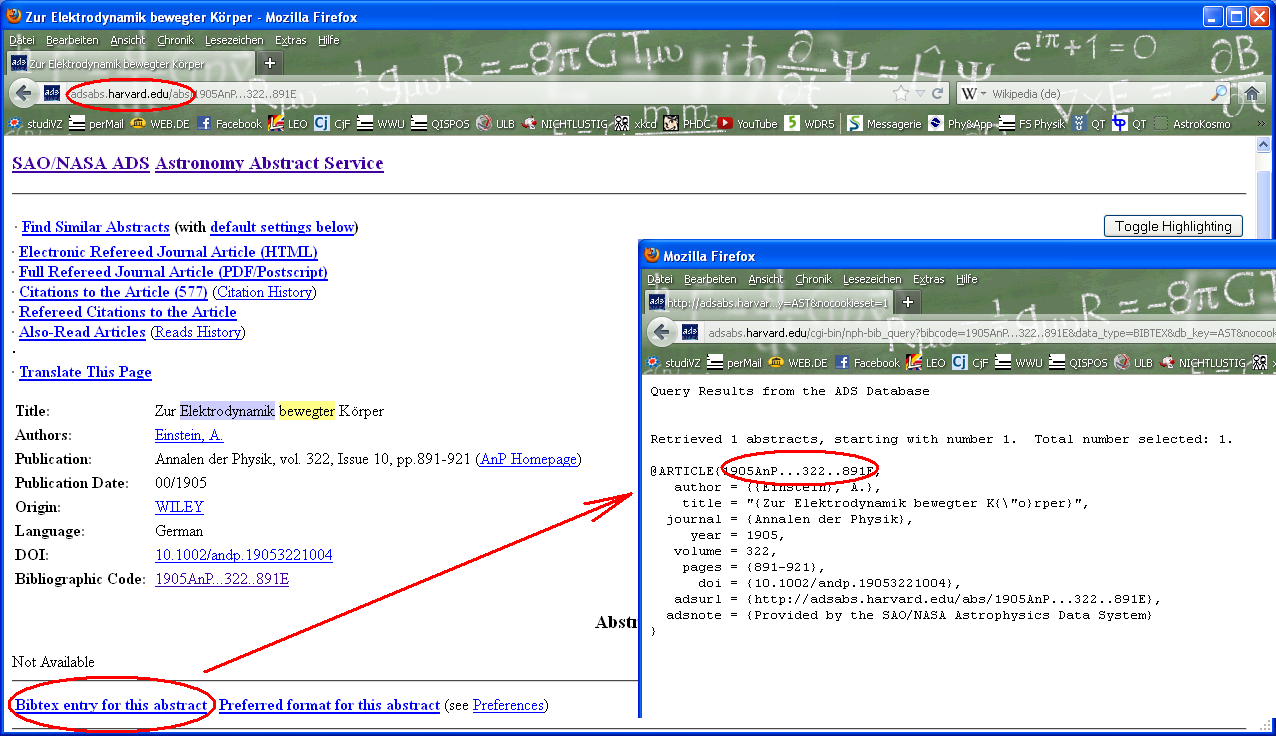
\includegraphics[width=1.00\textwidth]{adsabs}
\end{center}

Hier ist ganz viel Text und ein Zitat: (\verb+\cite{1905Einstein}+) \cite{1905Einstein}.

Das Programm $\verb+bibtex+$ erm�glicht es, Literaturangaben aus einer Datenbank (Textdatei mit Endung: .bib) zu holen.
Es werden im Literaturverzeichnis nur die Werke aufgef�hrt, die auch wirklich im Text zitiert werden.
Das Literarturverzeichnis selbst fordert man an mit:
\begin{verbatim}
\bibliographystyle{amsplain}
\bibliography{lit}
\end{verbatim}
Die Kompilierungsreihenfolge ist in diesem Fall:
\begin{itemize}

	\item
	pdflatex dateiname
	
	\item
	bibtex dateiname
	
	\item
	pdflatex dateiname

	\item
	pdflatex dateiname
	
\end{itemize}

\bibliographystyle{amsplain}
\bibliography{lit}


\end{document}